\documentclass{assignment}
\usepackage[pdftex]{graphicx}
\usepackage{xcolor}
\definecolor{LightGray}{gray}{0.95}
\usepackage{fancyvrb}
\usepackage{float}
\usepackage[letterpaper, margin = 2.5cm]{geometry}
\usepackage[T1]{fontenc}
\usepackage{amsmath, amsfonts, amssymb}
\usepackage{hyperref, url}
\usepackage{fancyhdr}
\usepackage{caption}
\captionsetup[figure]{labelformat=empty}

\newcommand{\n}{\vspace{0.2cm}}
\def\u{\mathbf u}
\def\v{\mathbf v}
\def\w{\mathbf w}
\def\x{\mathbf x}
\def\y{\mathbf y}
\def\z{\mathbf z}

\student{Fletcher Gornick}
\semester{Spring 2024}
\date{\today}

\courselabel{CSCI 5607}
\exercisesheet{Assignment 1B}{Lighting and Shading}

\school{College of Science and Engineering}
\university{University of Minnesota, Twin Cities}

\begin{document}

\begin{enumerate}
 \item Effects of \(O_{d \lambda}, O_{s \lambda}, k_a, k_d, k_s,\) and \(n\) on object illumination.
       \begin{itemize}
        \item \(O_{d \lambda}\): This is the objects underlying material color.  This is probably the most crucial part of the object's material.  If I were to ask you what color an object is, you'd respond with this.

        \item \(O_{s \lambda}\): This defines the color of the sheen on the object.  When an object is illuminated by an outside light source, this color will highlight the parts with more direct light.

        \item \(k_a\): This is the ambient reflection constant.  This defines the intensity of the base color of an object without any light shining on it.  This is a sort of fake mathematical constant that we use to simulate light rays not coming from any simulation-defined lights.  Increasing this will uniformly increase the intensity of an objects reflected light.

        \item \(k_d\): This is the diffuse reflection constant.  It scalse up the objects diffuse color anywhere that the surface normal is close to parallel with a light direction.  It basically says how much more intense to we want a color to be when light shines on it.

        \item \(k_s\): This is the specular reflection constant.  This tells us how intense we want an object to shine when hit by a light source.  Shinier objects have a larger \(k_s\).

        \item \(n\): This is the shininess constant.  Similar to the specular reflection constant, but this defines the dropoff in intensity.  For large \(n\), the dropoff in light intensity is very large, so an object will only appear shiny in a small spot.  For large \(n\) the shine will spread out further.
       \end{itemize}

       Below you can see an example where i tinker with each of the three reflection constants.

       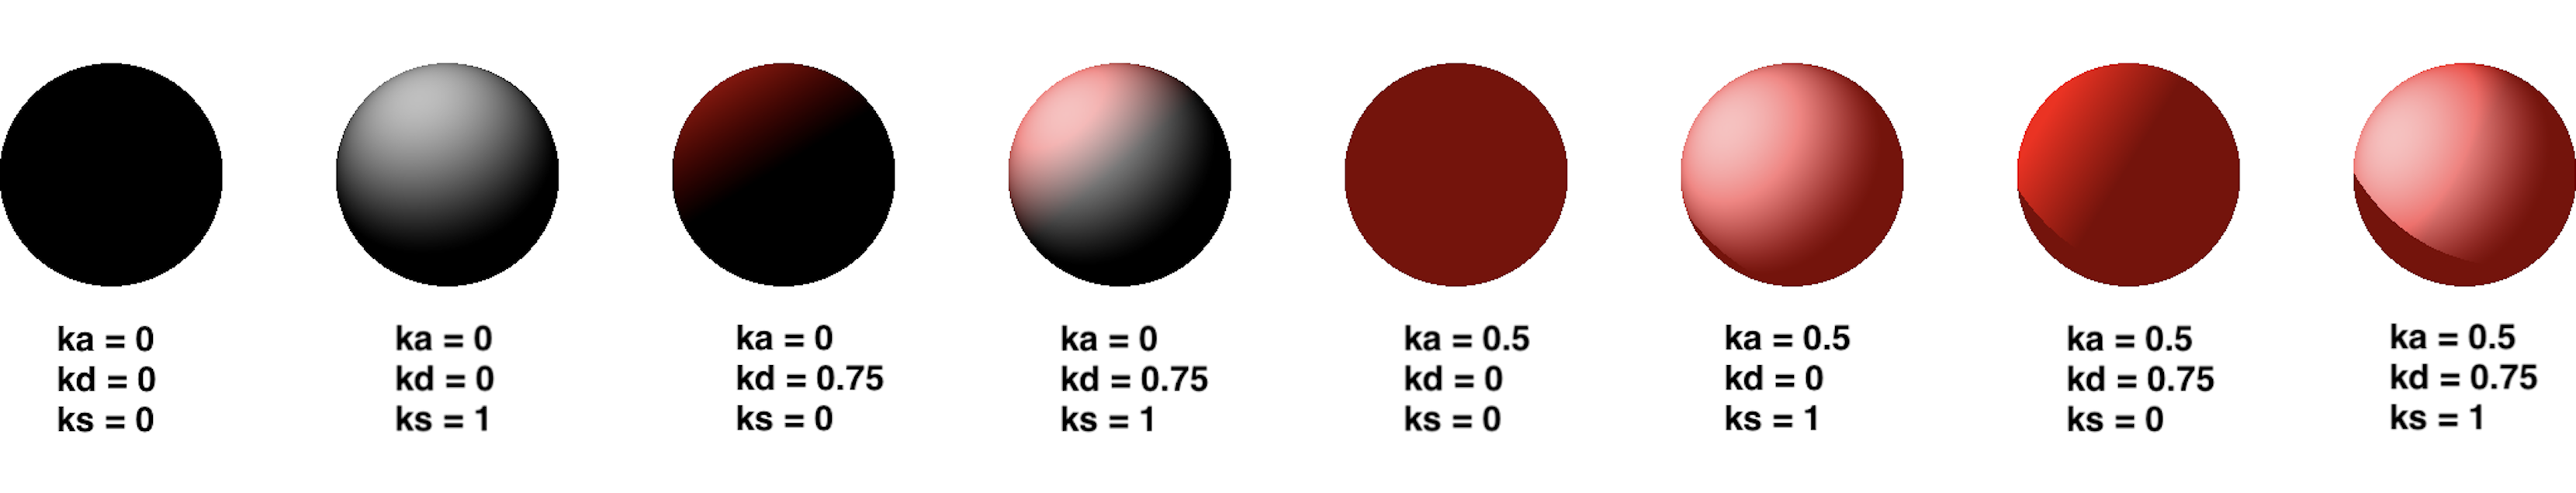
\includegraphics[width=15.5cm]{img/mtlcolor.png}

 \item Directional light source vs. point light source.

       This is very similar to how parallel projection differs from perspective projection (directional light source being more like parallel projection), only in the perspective of a light instead of the viewer.

       When shining completely perpendicular to objects, the shadow from a directional light is the exact size of the object, but when shooting more diagonally, light can become distorted.

       \begin{figure}[H]
        \centering
        \begin{minipage}[c]{0.23\linewidth}
         \centering
         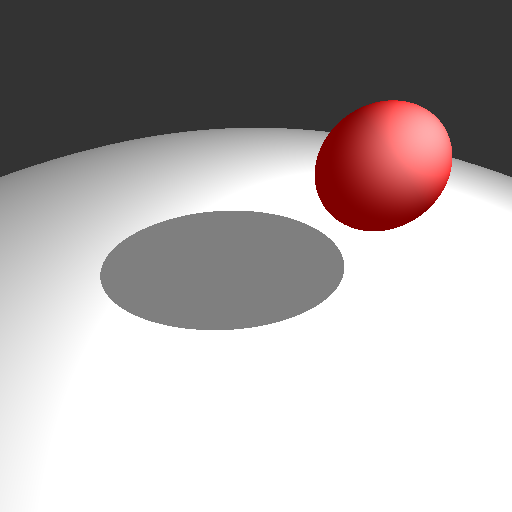
\includegraphics[width=3.5cm]{img/point_diag_light.png}
         \caption{\small{diagonal point light}}
        \end{minipage}
        \begin{minipage}[c]{0.23\linewidth}
         \centering
         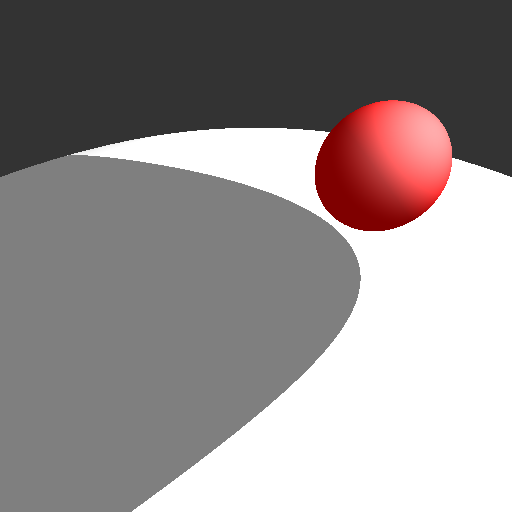
\includegraphics[width=3.5cm]{img/dir_diag_light.png}
         \caption{\small{diagonal directional light}}
        \end{minipage}
        \begin{minipage}[c]{0.23\linewidth}
         \centering
         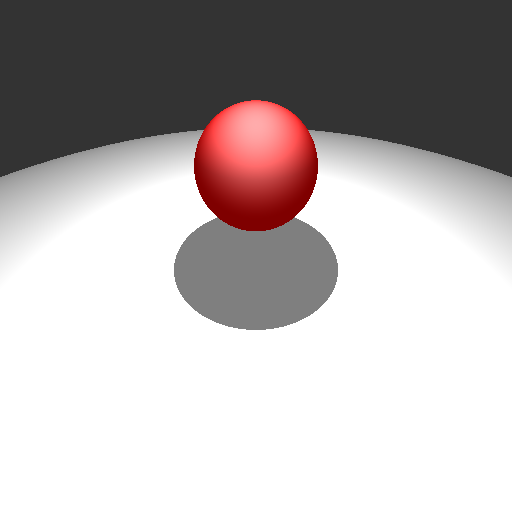
\includegraphics[width=3.5cm]{img/point_vert_light.png}
         \caption{\small{vertical point light}}
        \end{minipage}
        \begin{minipage}[c]{0.23\linewidth}
         \centering
         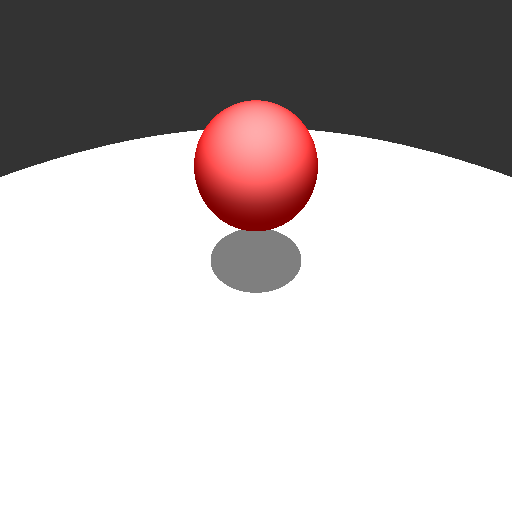
\includegraphics[width=3.5cm]{img/dir_vert_light.png}
         \caption{\small{vertical directional light}}
        \end{minipage}
       \end{figure}

 \item Use of multiple lights instead of a single light.

       Not much to add in this respect, adding more lights illuminates more surfaces.  One thing with multiple lights is that one part of an object can be in the shadow of another, while also recieving direct light from a different light source, leading to some cool overlaps.

       \begin{figure}[H]
        \centering
        \begin{minipage}[c]{0.46\linewidth}
         \centering
         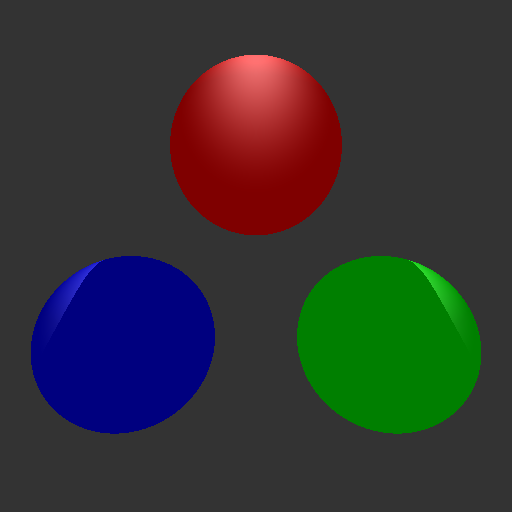
\includegraphics[width=7cm]{img/onelight.png}
         \caption{one light (above red)}
        \end{minipage}
        \begin{minipage}[c]{0.46\linewidth}
         \centering
         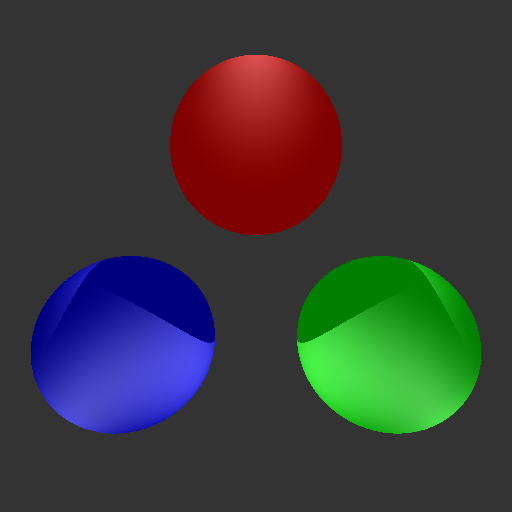
\includegraphics[width=7cm]{img/multiplelights.png}
         \caption{multiple lights}
        \end{minipage}
       \end{figure}

 \item EXTRA CREDIT: light source attenuation

       In reality, lights don't just reach every surface with the same intensity like this (light source is right in front of the middle ball)

       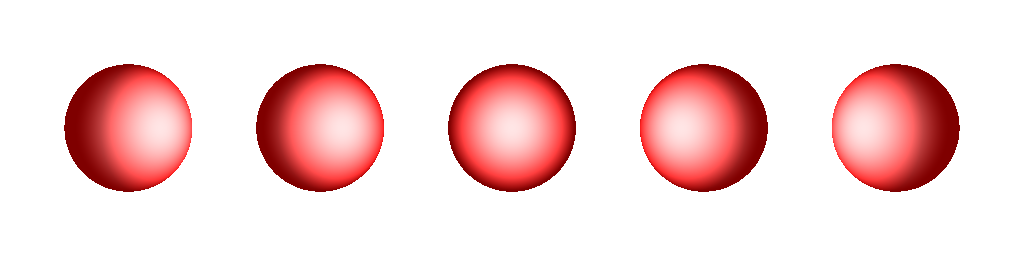
\includegraphics[width=14cm]{img/attenuation_before.png}

       but instead, the intensity of a light should reduce the further it travels through space like so...

       (\(c_1 = 0.2, \; c_2 = 0.1, \; c_3 = 0.05\))

       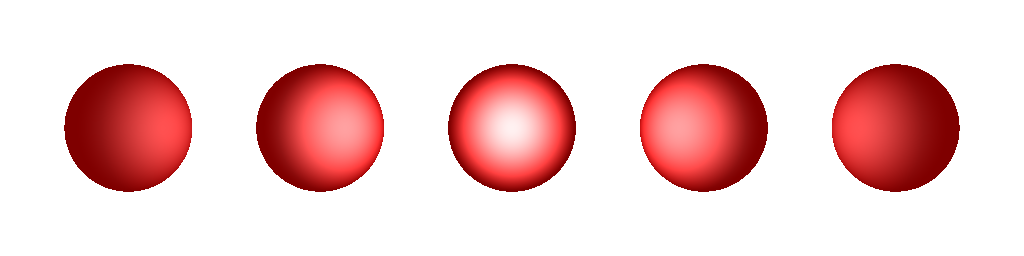
\includegraphics[width=14cm]{img/attenuation_after.png}

 \item EXTRA CREDIT: depth cueing.

       Another thing we can add to make our simulation look a bit more realistic is to implement depth cueing.  This makes it so objects further away from the viewer blend more into another color.  In this case I chose to make the depth cueing color match the background (example on next page).

       \begin{figure}[H]
        \centering
        \begin{minipage}[c]{0.46\linewidth}
         \centering
         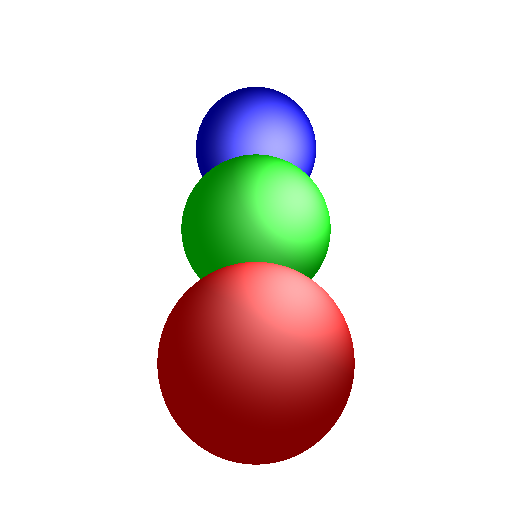
\includegraphics[width=7cm]{img/depthcueing_before.png}
         \caption{before depth cueing}
        \end{minipage}
        \begin{minipage}[c]{0.46\linewidth}
         \centering
         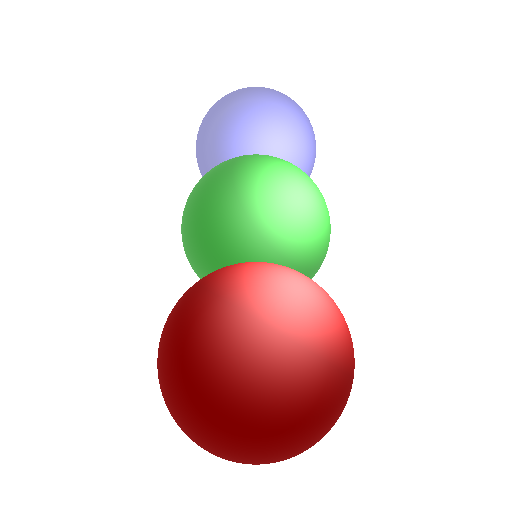
\includegraphics[width=7cm]{img/depthcueing_after.png}
         \caption{after: \(\alpha_{\text{min}} = 0.4, \;\; \alpha_{\text{max}} = 1.0\)}
        \end{minipage}
       \end{figure}

 \item EXTRA CREDIT: soft shadows

       The shadows on our simulation look a little too sharp to be realistic, and this is because our light sources are defined as single points.  In reality, light sources tend to come from an area instead, so if we add lights as invisible spheres in our simulation, and average out the illumination of rays shot from random points within the sphere, we can get more realistic looking shadows.

       \begin{figure}[H]
        \centering
        \begin{minipage}[c]{0.46\linewidth}
         \centering
         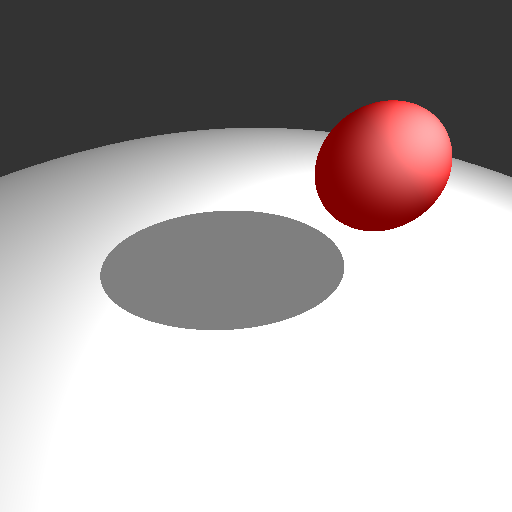
\includegraphics[width=7cm]{img/softshadows_before.png}
         \caption{before soft shadows}
        \end{minipage}
        \begin{minipage}[c]{0.46\linewidth}
         \centering
         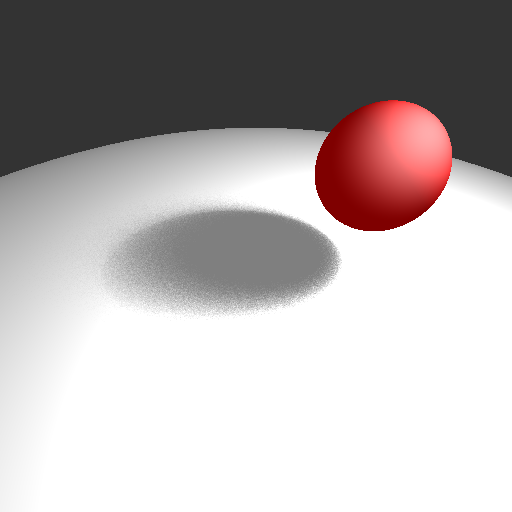
\includegraphics[width=7cm]{img/softshadows_after.png}
         \caption{after soft shadows (50 samples)}
        \end{minipage}
       \end{figure}
\end{enumerate}

\textbf{NOTE}: all these images were generated by the ray tracer I wrote in assignment 1B.  If you'd like to produce these images yourself, you can use the input files in the \verb|examples| folder.
\end{document}
